\part{Mathematics}

GNC is applied mathematics. Once you accept this the life will be easier. Once
you made your life easier you can make the decision whether going into applied
mathematics or not. Going into applied mathematics means accepting the
friendship of mathematical rigour. I made this decision and accepted that
mathematics is good and will be part of my life, and I write this book
accordingly.

The mathematics chapter includes a landscape of what mathematics is needed for
GNC in a graph form which is an information retrieval thesaurus. This help you
to see what is the study material and when you feel lost helps you to find the
"You are here!" point on this map.

The interesting part in mathematics comes after calculus. Everything before it
is just dead boring. But, these boring things are the air in the clouds of
Calculus, so that, you have to know these things.

\input{mathematics/thesaurus}

The below content is made based on Precalculus by James Stewart.

\chapter{Fundamentals}

\section{Real Numbers}

\section{Real Numbers - Anki cards}

%ankicard
%ankitags mathematics fundamentals precalculus
%ankifront
\begin{small}
    \begin{tabularx}{1\textwidth}{
            p{\dimexpr1\textwidth\relax}
        }
        \toprule
        \textbf{Real Numbers overview card} \\
        \toprule

        What does the numbers set structure look like? 
        \\
        \midrule

        What are the Natural numbers and its notation?
        \\
        \midrule

        What are the integers and its notation?
        \\
        \midrule

        What are the rational numbers and its notation?
        \\
        \midrule

        What are the irrational numbers and its notation?
        \\
        \midrule

        What are the properties of real numbers? (Commutative, Associative,
        Distributive)
        \\
        \midrule

        What are the rules of Addition and Subtraction?
        \\
        \midrule

        What are the rules of Multiplication and Division?
        \\
        \midrule

        What is the real line and its properties?
        \\
        \midrule

        What are the sets and intervals, its properties, notation and
        operations?
        \\
        \midrule

        What is absolute value and how it relates to distance?
        \\
        \midrule

        What are the properties of absolute value?
        \\
        \bottomrule

    \end{tabularx}
\end{small}
%ankifront end
%ankiback
\begin{small}
    \begin{tabularx}{1\textwidth}{
            p{\dimexpr1\textwidth\relax}
        }
        \toprule
        \textbf{Answers are on the subsequent cards in the topic} \\
        \toprule

    \end{tabularx}
\end{small}
%ankiback end

%ankicard
%ankitags mathematics fundamentals precalculus
\subsection{What does the numbers set structure look like?}
%ankifront
\begin{small}
    \begin{tabularx}{1\textwidth}{
            p{\dimexpr1\textwidth\relax}
        }
        \toprule
        \textbf{What does the numbers set structure look like?}\\
        \bottomrule

    \end{tabularx}
\end{small}
%ankifront end
%ankiback
\begin{small}
    \begin{tabularx}{1\textwidth}{
            p{\dimexpr1\textwidth\relax}
        }
        \toprule
        \textbf{The numbers set  structure looks like the following:} \\
        \midrule

        \makecell{
            Real numbers set, notation: $\mathbb{R}$, includes:\\
            Rational numbers, Notation: $ \mathbb{Q}; \text{ example: } \frac{4}{3}, 9.324$\\
            Irrational numbers, Notation: $ \mathbb{I}; \text{ example: } \sqrt{2} \pi $\\
            \\ 
            Rational numbers set includes:\\
            Integers, Notation: $\mathbb{Z} \text{ example: } -1, 2, 3, \cdots $\\
            \\
            Integers number set includes:\\
            Natural numbers, Notation: $\mathbb{N}, \text{ example: } 1, 2, 3 \cdots$
        }
        \\
        \bottomrule

    \end{tabularx}
\end{small}
%ankiback end

%ankicard
%ankitags mathematics fundamentals precalculus
\subsection{What are the Natural numbers and its notation?}
%ankifront
\begin{small}
    \begin{tabularx}{1\textwidth}{
            p{\dimexpr1\textwidth\relax}
        }
        \toprule
        What are the Natural numbers and its notation?
        \\
        \bottomrule

    \end{tabularx}
\end{small}
%ankifront end
%ankiback
\begin{small}
    \begin{tabularx}{1\textwidth}{
            p{\dimexpr1\textwidth\relax}
        }
        \toprule
            Natural numbers, Notation: $\mathbb{N}, \text{ example: } 1, 2, 3 \cdots$\\
        \bottomrule

    \end{tabularx}
\end{small}
%ankiback end

%ankicard
%ankitags mathematics fundamentals precalculus
\subsection{What are the Integers and its notation?}
%ankifront
\begin{small}
    \begin{tabularx}{1\textwidth}{
            p{\dimexpr1\textwidth\relax}
        }
        \toprule
        What are the integers and its notation?
        \\
        \bottomrule

    \end{tabularx}
\end{small}
%ankifront end
%ankiback
\begin{small}
    \begin{tabularx}{1\textwidth}{
            p{\dimexpr1\textwidth\relax}
        }
        \toprule
            Integers, Notation: $\mathbb{Z} \text{ example: } -1, 2, 3, \cdots $\\

    \end{tabularx}
\end{small}
%ankiback end

%ankicard
%ankitags mathematics fundamentals precalculus
\subsection{What are the Rational numbers and its notation?}
%ankifront
\begin{small}
    \begin{tabularx}{1\textwidth}{
            p{\dimexpr1\textwidth\relax}
        }
        \toprule
        What are the rational numbers and its notation?
        \\
        \bottomrule

    \end{tabularx}
\end{small}
%ankifront end
%ankiback
\begin{small}
    \begin{tabularx}{1\textwidth}{
            p{\dimexpr1\textwidth\relax}
        }
        \toprule
        Rational numbers, Notation: $ \mathbb{Q}; \text{ example: } \frac{4}{3}, 9.324$\\
        \bottomrule

    \end{tabularx}
\end{small}
%ankiback end

%ankicard
%ankitags mathematics fundamentals precalculus
\subsection{What are the Irrational numbers and its notation?}
%ankifront
\begin{small}
    \begin{tabularx}{1\textwidth}{
            p{\dimexpr1\textwidth\relax}
        }
        \toprule
        What are the irrational numbers and its notation?
        \\
        \bottomrule

    \end{tabularx}
\end{small}
%ankifront end
%ankiback
\begin{small}
    \begin{tabularx}{1\textwidth}{
            p{\dimexpr1\textwidth\relax}
        }
        \toprule
        Irrational numbers, Notation: $ \mathbb{I}; \text{ example: } \sqrt{2}, \pi $\\
        \bottomrule

    \end{tabularx}
\end{small}
%ankiback end

%ankicard
%ankitags mathematics algebra precalculus
\subsection{What are the properties of Real Numbers?}

%ankifront
\begin{small}
\begin{tabularx}{1\textwidth}{
    p{\dimexpr1\textwidth\relax}
}
\toprule
\textbf{What are the properties of Real Numbers?} \\
\midrule
\end{tabularx}
\end{small}

%ankifront end
%ankiback
\begin{small}
    \begin{tabularx}{1\textwidth}{
            p{\dimexpr1\textwidth\relax}
        }
        \toprule
        Properties of Real Numbers \\
        \midrule


\makecell[l]{
    \textbf{Commutative Properties} \\ 1[ex]
    $a + b = b + a$ \\ 
    $a \cdot b = b \cdot a$
} 
\\
\midrule

\makecell[l]{
    \textbf{Associative Properties} \\[1ex] 
    $(a + b) + c = a + (b + c)$ \\ 
    $(a \cdot b) \cdot c = a \cdot (b \cdot c)$
} 
\\

\midrule

\makecell[l]{
    \textbf{Distributive Properties} \\[1ex] 
    $a(b + c) = a \cdot b + a \cdot c$ \\ 
    $(b + c) \cdot a = a \cdot b + a \cdot c$
} 
\\  

\bottomrule
\end{tabularx}
\end{small}
%ankiback end

%ankicard
%ankitags mathematics algebra precalculus
\subsection{What are the properties of Addition and Subtraction?}

%ankifront
\begin{small}
    \begin{tabularx}{1\textwidth}{
        p{\dimexpr1\textwidth\relax}
    }
        \toprule
        \textbf{What are the properties of Addition and Subtraction?} \\
        \bottomrule
    \end{tabularx}
\end{small}
%ankifront end

%ankiback
\begin{small}
    \begin{tabularx}{1\textwidth}{
            p{\dimexpr1\textwidth\relax}
        }
        \toprule
        Properties of Addition and Subtraction \\
        \midrule

        \makecell[l]{
            $(-1)a = -a$
        } 
        \\

        \makecell[l]{
            $-(-a) = a$
        } 
        \\
        \makecell[l]{
            $(-a)b = a(-b) = -(ab)$
        } 
        \\
        \makecell[l]{
            $(-a)(-b) = ab$
        } 
        \\
        \makecell[l]{
            $-(a+b) = -a-b$
        } 
        \\
        \makecell[l]{
            $-(a-b) = b-a = -a + b$
        } 
        \\
        \bottomrule
    \end{tabularx}
\end{small}
%ankiback end

%ankicard
%ankitags mathematics algebra precalculus
\subsection{What are the properties of Multiplication and Division?}

%ankifront
\begin{small}
    \begin{tabularx}{1\textwidth}{
        p{\dimexpr1\textwidth\relax}
    }
        \toprule
        \textbf{What are the Rules of Multiplication and Division?} \\
        \midrule
    \end{tabularx}
\end{small}
%ankifront end

%ankiback
\begin{small}
    \begin{tabularx}{1\textwidth}{
            p{\dimexpr1\textwidth\relax}
        }

        \textbf{Properties of Multiplication and Division} \\
    \midrule

    \makecell[l]{
        \vspace{5pt}
        1, $ \frac{a}{b} \cdot \frac{c}{d} = \frac{ac}{bd} $
        \vspace{5pt}
    } 
    \\
    \makecell[l]{
        \vspace{5pt}
    2, $ \frac{a}{b} \div \frac{c}{d} = \frac{a}{b} \cdot \frac{d}{c} $
        \vspace{5pt}
    } 
    \\
    \makecell[l]{
        \vspace{5pt}
    3, $ \frac{a}{c} + \frac{b}{c} = \frac{a + b}{c} $
        \vspace{5pt}
    } 
    \\
    \makecell[l]{
        \vspace{5pt}
    4, $ \frac{a}{b} + \frac{c}{d} = \frac{ad + cb}{bd} $
        \vspace{5pt}
    } 
    \\
    \makecell[l]{
        \vspace{5pt}
        5,  $ \frac{ac}{bc} = \frac{a}{b} $
        \vspace{5pt}
    } 
    \\
    \makecell[l]{
        \vspace{5pt}
    6, $ \text{If } \frac{a}{b} = \frac{c}{d}, \text{then } ad = bc$
        \vspace{5pt}
    } 
    \\
    \bottomrule
    \end{tabularx}
\end{small}
%ankiback end

%ankicard
%ankitags mathematics algebra precalculus
\subsection{What are the properties of the Real Line?}

%ankifront
\begin{small}
    \begin{tabularx}{1\textwidth}{
            p{\dimexpr1\textwidth\relax}
        }
        \toprule
        \textbf{What are the the properties of the Real Line?} \\
        \bottomrule
    \end{tabularx}
\end{small}
%ankifront end

%ankiback
\begin{small}
\begin{tabularx}{1\textwidth}{
        p{\dimexpr0.5\textwidth\relax}
        p{\dimexpr0.5\textwidth\relax}
    }
    \toprule
    \multicolumn{2}{c}{\textbf{Properties of the Real Line}} \\
    \midrule

    \textbf{Property} & \textbf{Details}\\
    \midrule

    Reference point, origin & Its value is $0$ \\
    \midrule

    Positive numbers & Right side of the reference point \\
    \midrule

    Negative numbers & Left side of the reference point \\
    \midrule

    Order & the real numbers are ordered in the Real Line \\
    \bottomrule

\end{tabularx}
\end{small}
%ankiback end

%ankicard
%ankitags mathematics algebra precalculus
\subsection{What are the notations of Sets and Intervals?}
%ankifront

\begin{small}
    \begin{tabularx}{1\textwidth}{
        p{\dimexpr1\textwidth\relax}
    }
    \toprule
    \textbf{What are the notations of Sets and Intervals?}
    \\
    \bottomrule
    \end{tabularx}
\end{small}
%ankifront end
%ankiback

\begin{small}
\begin{tabularx}{1\textwidth}{
        p{\dimexpr0.5\textwidth\relax}
        p{\dimexpr0.5\textwidth\relax}
    }
    \toprule
    \multicolumn{2}{c}{\textbf{Notations of Sets and Intervals}} \\
    \midrule
    \multicolumn{2}{l}{
        A \textbf{Set} is a collection of objects called \textbf{elements}
    } \\
    \midrule
    $S$ & sign of a Set \\
    \midrule
    $a \in S$ & $a$ is element of $S$ \\
    \midrule
    $b \notin S$  & $b$ is not element of $S$ \\
    \midrule
    $S \cup T$  & union of $S$ and $T$ sets \\
    \midrule
    $S \cap T$ & intersection of $S$ and $T$ sets \\
    \midrule
    $\emptyset$ & empty set \\
    \midrule
    $A = \{1, 2, 3, 4, 5\}$ & the listing elements notation of a Set \\
    \midrule
    $ A = \{x | x \text{ is an integer and } 0 < x < 8 \}$ &
    the builder notation \\
    \bottomrule
\end{tabularx}
\end{small}
%ankiback end

%ankicard
%ankitags mathematics algebra precalculus
\subsection{What are the notations of intervals?}
%ankifront

\begin{small}
    \begin{tabularx}{1\textwidth}{
        p{\dimexpr1\textwidth\relax}
    }
    \toprule
    \textbf{What are the notations of intervals?} \\
    \bottomrule
    \end{tabularx}
\end{small}
%ankifront end
%ankiback

\begin{small}
\begin{tabularx}{1\textwidth}{
    p{\dimexpr0.3\textwidth\relax}
    p{\dimexpr0.3\textwidth\relax}
    p{\dimexpr0.4\textwidth\relax}
}
\toprule
Notation & Set Description & Graph \\
\midrule

$ \left( a,b \right) $ &
$ \left\{ x | a < x < b \right\} $ &
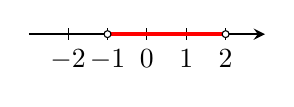
\begin{tikzpicture}[scale=0.5]
  % Drawing the real number line
  \draw[thick, -stealth] (-3,0) -- (3,0); % Main line with arrow
  \foreach \x in {-2,-1,0,1,2} {
    \draw (\x,0.15) -- (\x,-0.15) node[below] {$\x$}; % Tick marks and labels
  }
  % \draw (0,0.3) -- (0,-0.3) node[below] {$0$}; % Emphasize origin

  % Marking the interval [-2, 3)
  \draw[line width=1.5pt, red] (-1,0) -- (2,0); % Thick line for interval
  \draw[black, fill=white] (-1,0) circle (2.5pt); % Closed endpoint at -2
  \draw[black, fill=white] (2,0) circle (2.5pt); % Open endpoint at 3
\end{tikzpicture}
\\
\midrule

$ \lbrack a,b \rbrack $ &
$ \left\{ x | a \leq x \leq b \right\} $ &
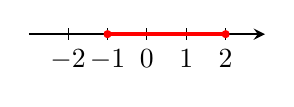
\begin{tikzpicture}[scale=0.5]
  % Drawing the real number line
  \draw[thick, -stealth] (-3,0) -- (3,0); % Main line with arrow
  \foreach \x in {-2,-1,0,1,2} {
    \draw (\x,0.15) -- (\x,-0.15) node[below] {$\x$}; % Tick marks and labels
  }
  % \draw (0,0.3) -- (0,-0.3) node[below] {$0$}; % Emphasize origin

  % Marking the interval [-2, 3)
  \draw[line width=1.5pt, red] (-1,0) -- (2,0); % Thick line for interval
  \filldraw[red] (-1,0) circle (2.5pt); % Closed endpoint at -2
  \filldraw[red] (2,0) circle (2.5pt); % Open endpoint at 3
\end{tikzpicture}
\\
\midrule

$ \lbrack a,b ) $ &
$ \left\{ x | a \leq x < b \right\} $ &
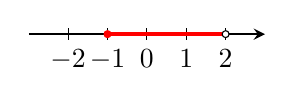
\begin{tikzpicture}[scale=0.5]
  % Drawing the real number line
  \draw[thick, -stealth] (-3,0) -- (3,0); % Main line with arrow
  \foreach \x in {-2,-1,0,1,2} {
    \draw (\x,0.15) -- (\x,-0.15) node[below] {$\x$}; % Tick marks and labels
  }
  % \draw (0,0.3) -- (0,-0.3) node[below] {$0$}; % Emphasize origin

  % Marking the interval [-2, 3)
  \draw[line width=1.5pt, red] (-1,0) -- (2,0); % Thick line for interval
  \filldraw[red] (-1,0) circle (2.5pt); % Closed endpoint at -2
  \draw[black, fill=white] (2,0) circle (2.5pt); % Open endpoint at 3
\end{tikzpicture}
\\

\midrule
$ ( a,b \rbrack $ &
$ \left\{ x | a < x \leq b \right\} $ &
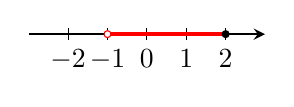
\begin{tikzpicture}[scale=0.5]
  % Drawing the real number line
  \draw[thick, -stealth] (-3,0) -- (3,0); % Main line with arrow
  \foreach \x in {-2,-1,0,1,2} {
    \draw (\x,0.15) -- (\x,-0.15) node[below] {$\x$}; % Tick marks and labels
  }
  % \draw (0,0.3) -- (0,-0.3) node[below] {$0$}; % Emphasize origin

  % Marking the interval [-2, 3)
  \draw[line width=1.5pt, red] (-1,0) -- (2,0); % Thick line for interval
  \draw[red, fill=white] (-1,0) circle (2.5pt); % Closed endpoint at -2
  \filldraw[black] (2,0) circle (2.5pt); % Open endpoint at 3
\end{tikzpicture}
\\
\midrule

$ ( a,\infty ) $ &
$ \left\{ x | a < \infty \right\} $ &
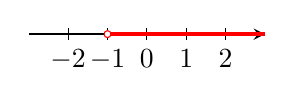
\begin{tikzpicture}[scale=0.5]
  % Drawing the real number line
  \draw[thick, -stealth] (-3,0) -- (3,0); % Main line with arrow
  \foreach \x in {-2,-1,0,1,2} {
    \draw (\x,0.15) -- (\x,-0.15) node[below] {$\x$}; % Tick marks and labels
  }
  % \draw (0,0.3) -- (0,-0.3) node[below] {$0$}; % Emphasize origin

  % Marking the interval [-2, 3)
  \draw[line width=1.5pt, red] (-1,0) -- (3,0); % Thick line for interval
  \draw[red, fill=white] (-1,0) circle (2.5pt); % Closed endpoint at -2
  % \filldraw[black] (2,0) circle (2.5pt); % Open endpoint at 3
\end{tikzpicture}
\\
\midrule

$ \lbrack a,\infty ) $ &
$ \left\{ x | a \leq \infty \right\} $ &
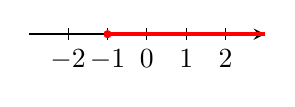
\begin{tikzpicture}[scale=0.5]
  % Drawing the real number line
  \draw[thick, -stealth] (-3,0) -- (3,0); % Main line with arrow
  \foreach \x in {-2,-1,0,1,2} {
    \draw (\x,0.15) -- (\x,-0.15) node[below] {$\x$}; % Tick marks and labels
  }
  % \draw (0,0.3) -- (0,-0.3) node[below] {$0$}; % Emphasize origin

  % Marking the interval [-2, 3)
  \draw[line width=1.5pt, red] (-1,0) -- (3,0); % Thick line for interval
  \filldraw[red] (-1,0) circle (2.5pt); % Closed endpoint at -2
  % \filldraw[black] (2,0) circle (2.5pt); % Open endpoint at 3
\end{tikzpicture}
\\
\midrule

$ ( -\infty, a ) $ &
$ \left\{ x | x < a \right\} $ &
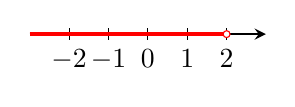
\begin{tikzpicture}[scale=0.5]
  % Drawing the real number line
  \draw[thick, -stealth] (-3,0) -- (3,0); % Main line with arrow
  \foreach \x in {-2,-1,0,1,2} {
    \draw (\x,0.15) -- (\x,-0.15) node[below] {$\x$}; % Tick marks and labels
  }
  % \draw (0,0.3) -- (0,-0.3) node[below] {$0$}; % Emphasize origin

  % Marking the interval [-2, 3)
  \draw[line width=1.5pt, red] (-3,0) -- (2,0); % Thick line for interval
  \draw[red, fill=white] (2,0) circle (2.5pt); % Closed endpoint at -2
  % \filldraw[black] (2,0) circle (2.5pt); % Open endpoint at 3
\end{tikzpicture}
\\
\midrule

$ ( -\infty, a \rbrack $ &
$ \left\{ x | x \leq a \right\} $ &
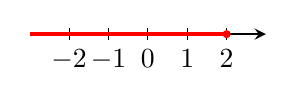
\begin{tikzpicture}[scale=0.5]
  % Drawing the real number line
  \draw[thick, -stealth] (-3,0) -- (3,0); % Main line with arrow
  \foreach \x in {-2,-1,0,1,2} {
    \draw (\x,0.15) -- (\x,-0.15) node[below] {$\x$}; % Tick marks and labels
  }
  % \draw (0,0.3) -- (0,-0.3) node[below] {$0$}; % Emphasize origin

  % Marking the interval [-2, 3)
  \draw[line width=1.5pt, red] (-3,0) -- (2,0); % Thick line for interval
  \filldraw[red] (2,0) circle (2.5pt); % Closed endpoint at -2
  % \filldraw[black] (2,0) circle (2.5pt); % Open endpoint at 3
\end{tikzpicture}
\\
\midrule

$ ( -\infty, \infty ) $ &
$ \mathbb{R} \text{set of real numbers} $ &
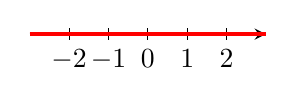
\begin{tikzpicture}[scale=0.5]
  % Drawing the real number line
  \draw[thick, -stealth] (-3,0) -- (3,0); % Main line with arrow
  \foreach \x in {-2,-1,0,1,2} {
    \draw (\x,0.15) -- (\x,-0.15) node[below] {$\x$}; % Tick marks and labels
  }
  % \draw (0,0.3) -- (0,-0.3) node[below] {$0$}; % Emphasize origin

  % Marking the interval [-2, 3)
  \draw[line width=1.5pt, red] (-3,0) -- (3,0); % Thick line for interval
  % \filldraw[red] (2,0) circle (2.5pt); % Closed endpoint at -2
  % \filldraw[black] (2,0) circle (2.5pt); % Open endpoint at 3
\end{tikzpicture}
\\
\midrule

\end{tabularx}
\end{small}
%ankiback end

%ankicard
%ankitags mathematics, fundamentals, modeling_with_equations
\subsection{
What are the absolute value inequalities?}
%ankifront
\begin{small}
    \begin{tabularx}{1\textwidth}{
            p{\dimexpr1\textwidth\relax}
        }
        \toprule
        What are the absolute value inequalities?
        \\
        \bottomrule
    \end{tabularx}
\end{small}
%ankifront end
%ankiback
\begin{small}
    \begin{tabularx}{1\textwidth}{
            p{\dimexpr1\textwidth\relax}
        }
        \toprule
        When absolute value is involved in inequalities it includes both the
        positive and negative numbers.
        \\
        \bottomrule
    \end{tabularx}
\end{small}
%ankiback end

%ankicard
%ankitags mathematics algebra precalculus
\subsection{Distance of two points on the Real Line}
%ankifront
\begin{small}
    \begin{tabularx}{1\textwidth}{
            p{\dimexpr1\textwidth\relax}
        }
        \toprule
        \textbf{Distance of two points on the Real Line} \\
        \bottomrule
    \end{tabularx}
\end{small}
%ankifront end

%ankiback

% \begin{small}
\begin{tabularx}{1\textwidth}{
        p{\dimexpr0.5\textwidth\relax}
        p{\dimexpr0.5\textwidth\relax}
    }
\toprule
\multicolumn{2}{c}{\textbf{Distance between two points}} \\
\midrule

$ d(a, b) = \left| b - a \right| $ &
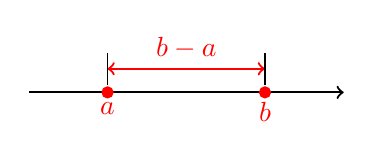
\begin{tikzpicture}
    % Draw the line
    \draw[thick, ->] (0,0) -- (4,0);
    
    % Draw points
    \filldraw[red] (1,0) circle (2pt) node[below] {$a$};
    \filldraw[red] (3,0) circle (2pt) node[below] {$b$};
    
    % Draw the vector
    \draw[red, thick, <->] (1,0.3) -- (3,0.3) node[midway, above] {$ \lvert b - a \rvert $};
    \draw[black] (1,0.1) -- ++(0,0.4);
    \draw[black] (3,0.1) -- ++(0,0.4);
    % \draw[red, thick, <-] (0,-0.2) -- (4,-0.2);
\end{tikzpicture}
\\
\bottomrule


\end{tabularx}
% \end{small}
%ankiback end


\section{Exponents and Radicals}

\section{Exponents and Radicals - Ankicards}

%ankicard
%ankitags mathematics precalculus
\subsection{What are the details of Rational Expressions?}
%ankifront
\begin{small}
    \begin{tabularx}{1\textwidth}{
            p{\dimexpr1\textwidth\relax}
        }
        \toprule
        \textbf{What are the details of Rational Expressions?}
        \\
        \midrule

        What is the domain of an algebraic expression?
        \\
        \midrule

        How to find the domain of an algebraic expression?
        \\
        \midrule

        What are the rules of simplyfing algebraic expressions?
        \\
        \bottomrule

    \end{tabularx}
\end{small}
%ankifront end
%ankiback
\begin{small}
    \begin{tabularx}{1\textwidth}{
            p{\dimexpr1\textwidth\relax}
        }
        \toprule
        Answers are in the subsequent cards in the topic
        \\
        \bottomrule

    \end{tabularx}
\end{small}
%ankiback end

%ankicard
%ankitags mathematics precalculus
\subsection{What are the details of exponents and radicals?}

%ankifront
\begin{small}
    \begin{tabularx}{1\textwidth}{
            p{\dimexpr1\textwidth\relax}
        }
        \toprule
        \textbf{What are the integer exponents?} \\
        \bottomrule
    \end{tabularx}
\end{small}

%ankifront end
%ankiback
\begin{small}
    \begin{tabularx}{1\textwidth}{
            p{\dimexpr1\textwidth\relax}
        }
        \toprule
        \makecell{
        If $a$ is any real number and $n$ is a positive integer, then the n-th
        power or $a$ is:\\
        $a^n = a \cdot a \cdot \cdots \cdot a$\\
        The number $a$ is called the base, and $n$ is called the exponent.
        }
        \\
        \bottomrule
    \end{tabularx}
\end{small}

%ankiback end

%ankicard
%ankitags mathematics precalculus
\subsection{What are the details of exponents and radicals?}

%ankifront
\begin{small}
    \begin{tabularx}{1\textwidth}{
            p{\dimexpr1\textwidth\relax}
        }
        \toprule
        What is the notation of zero and negative exponents?
        \\
        \bottomrule

    \end{tabularx}
\end{small}

%ankifront end
%ankiback
\begin{small}
    \begin{tabularx}{1\textwidth}{
            p{\dimexpr1\textwidth\relax}
        }
        \toprule
        $ a^{0} = 1 \text{ and } a^{-n}  = \frac{1}{a^{n}} $
        \\
        \bottomrule
    \end{tabularx}
\end{small}

%ankiback end

%ankicard
%ankitags mathematics algebra precalculus

\subsection{What are the rules of exponents?}

%ankifront
\begin{small}
    \begin{tabularx}{1\textwidth}{
            p{\dimexpr1\textwidth\relax}
        }
        \toprule
        What are the rules of exponents?
        \\
        \bottomrule

    \end{tabularx}
\end{small}
%ankifront end

%ankiback

\begin{small}
\begin{tabularx}{1\textwidth}{
    p{\dimexpr0.3\textwidth\relax}
    p{\dimexpr0.7\textwidth\relax}
}
\toprule
\multicolumn{2}{c}{\textbf{Laws of Exponents}} \\
\midrule

Rule & Explanation \\
\midrule

$ a^{0} = 1 \text{ and } a^{-n}  = \frac{1}{a^{n}} $
&
If $a \neq 0$ is a real number and $n$ is a positive integer
\\

\midrule

$ a^{m} \cdot a^{n} = a^{m + n} $ & \\
\midrule

$ \frac{a^{m}}{a^{n}} = a^{m-n} $ & \\
\midrule

$ \left( a^{m} \right)^{n} = a^{m \cdot n} $ & \\
\midrule

$ \left( ab \right)^{n} = a^{n} \cdot b^{n} $ & \\
\midrule

$ \left( \frac{a}{b} \right) ^{n} = \frac{a^{n}}{b^{n}} $ & \\
\midrule

$ \left( \frac{a}{b} \right)^{-n} = \left( \frac{b}{a} \right)^{n} $ & \\
\midrule

$ \frac{a^{-m}}{b^{-n}} = \frac{b^{n}}{a^{m}} $ & \\
\bottomrule

\end{tabularx}
\end{small}
%ankiback end

%ankicard
%ankitags mathematics precalculus
\subsection{How to use exponents laws to simplify expressions?}

%ankifront
\begin{small}
    \begin{tabularx}{1\textwidth}{
            p{\dimexpr1\textwidth\relax}
        }
        \toprule
        How to use the laws of Exponents to simplify expressions and expressions
        with negative exponents?
        \\
        \bottomrule

    \end{tabularx}
\end{small}

%ankifront end
%ankiback
\begin{small}
\begin{tabularx}{1\textwidth}{
        p{\dimexpr1\textwidth\relax}
    }
    \toprule
        \begin{multline*}
            \left(2a^3 b^2\right)\left(3a b^4\right) = \left(2a^3b^2\right)\lbrack 3^3a^3\left(b^4\right)^3\rbrack
            \rightarrow \text{ Law 4 }: \left(ab\right)^n = a^nb^n \\
            = \left(2a^3b^2\right)\left(27a^3b^12\right) 
            \rightarrow \text{ Law 3 }:
            \left(a^m\right)^n = a^{m \cdot n} \\
            = \left(2\right)\left(27\right)a^3a^3b^2b^{12}
            \rightarrow \text{ Group factors with the same base } \\
            = 54a^6b{14} \rightarrow \text{ Law 1: } a^m \cdot a^n = a^{m+n} \\
        \end{multline*}
        \\
        \midrule
        \begin{multline*}
            \frac{6st^{-4}}{2s^{-2}t^2} = \frac{6ss^2}{2t^2t^4} \rightarrow
            \text{ Law 7 } \\
            = \frac{3s^3}{t^6} \rightarrow \text{ Law 1 } \\
        \end{multline*}
        \\
    \bottomrule
\end{tabularx}
\end{small}
%ankiback end

%ankicard
%ankitags mathematics algebra precalculus

%ankifront
\begin{small}
    \begin{tabularx}{1\textwidth}{
            p{\dimexpr1\textwidth\relax}
        }
        \toprule
        What are the details of scientific notation?
        \\
        \bottomrule
    \end{tabularx}
\end{small}
%ankifront end

%ankiback
\begin{small}
\begin{tabularx}{1\textwidth}{
        p{\dimexpr0.5\textwidth\relax}
        p{\dimexpr0.5\textwidth\relax}
    }
    \toprule
    \multicolumn{2}{c}{Details of Scientific Notation} \\
    \midrule

    $ x = a \times 10^n $ 
    & where $1 \leq a < 10 \text{ and } n \text{ is an integer } $
    \\
    \bottomrule

\end{tabularx}
\end{small}
%ankiback end

%ankicard
%ankitags mathematics precalculus
%ankifront
\begin{small}
    \begin{tabularx}{1\textwidth}{
            p{\dimexpr1\textwidth\relax}
        }
        \toprule
        What are the radicals and what is the definition of n-th root?
        \\
        \bottomrule

    \end{tabularx}
\end{small}

%ankifront end
%ankiback
\begin{small}
    \begin{tabularx}{1\textwidth}{
            p{\dimexpr1\textwidth\relax}
        }
        \toprule
        \makecell{
            \textbf{Definition of n-th Root}\\
            If $n$ is any positive integer, then the principal n-th root of $a$
            is defined as follows:\\
            $\sqrt[n]{a} \text{ means } b^n = a $\\
            If $n$ is even, then we must have $a \geq 0 \text{ and } b \geq 0$\\
        }
        \\
        \bottomrule
    \end{tabularx}
\end{small}

%ankiback end

%ankicard
%ankitags mathematics algebra precalculus

%ankifront
\begin{small}
    \begin{tabularx}{1\textwidth}{
            p{\dimexpr1\textwidth\relax}
        }
        \toprule
        What are the Laws of Roots?
        \\
        \bottomrule

    \end{tabularx}
\end{small}
%ankifront end

%ankiback
\begin{tabularx}{1\textwidth}{
        p{\dimexpr0.5\textwidth\relax}
        p{\dimexpr0.5\textwidth\relax}
    }
    \toprule
    \multicolumn{2}{c}{\textbf{Laws of Roots}} \\
    \midrule
    $ \sqrt[n]{ab} = \sqrt[n]{a} \cdot \sqrt[n]{b} $ & \\
    \midrule

    $ \sqrt[n]{ \frac{a}{b} } = \frac{ \sqrt[n]{a} }{ \sqrt[n]{a} } $ & \\
    \midrule

    $ \sqrt[n]{ \sqrt[m]{a}} = \sqrt[n \cdot m]{a} $ & \\
    \midrule

    $ \sqrt[n]{ a^{n} } = a, \text{ if } n \text{ odd } $ & \\
    \midrule

    $ \sqrt[n]{ a^{n} } = \lvert a \rvert, \text{ if } n \text{ is even } $ &
    \\
    \midrule

    $ a^{ \frac{1}{n} } = \sqrt[n]{a} $ & \\
    \midrule

    $ a^{ \frac{m}{n} } = \sqrt[n]{ a^{m} } $ & \\
    \bottomrule
\end{tabularx}
%ankiback end

%ankicard
%ankitags mathematics precalculus
%ankifront
\begin{small}
    \begin{tabularx}{1\textwidth}{
            p{\dimexpr1\textwidth\relax}
        }
        \toprule
        How to combine radicals and how not to?
        \\
        \bottomrule

    \end{tabularx}
\end{small}

%ankifront end
%ankiback
\begin{small}
    \begin{tabularx}{1\textwidth}{
            p{\dimexpr1\textwidth\relax}
        }
        \toprule
        \makecell{
            \textbf{Positive case}\\
            $ \sqrt{32} + \sqrt{200} = \sqrt{16 \cdot 2} + \sqrt{100 \cdot 2} $\\
            $ = \sqrt{16}\sqrt{2} + \sqrt{100}\sqrt{2} $\\
            $ = 4\sqrt{2} + 10\sqrt{2} $\\
            $ = 14\sqrt{2} $\\
        }
        \\
        \midrule
        \makecell{
            \textbf{Negative case}\\
            $ \text{WRONG!!! } \sqrt{a + b} = \sqrt{a} + \sqrt{b} \text{ WRONG!!! } $\\
        }
        \\
        \bottomrule
    \end{tabularx}
\end{small}

%ankiback end

%ankicard
%ankitags mathematics precalculus
%ankifront
\begin{small}
    \begin{tabularx}{1\textwidth}{
            p{\dimexpr1\textwidth\relax}
        }
        \toprule
        What are the rational exponents and what is the definition?
        \\
        \bottomrule
    \end{tabularx}
\end{small}

%ankifront end
%ankiback
\begin{small}
    \begin{tabularx}{1\textwidth}{
            p{\dimexpr1\textwidth\relax}
        }
        \toprule
        \makecell{
            $ a^{\frac{1}{n}} = \sqrt[n]{a} $\\
            \\
            For any rational exponent $m/n$ in lowest terms,\\ 
            where $m$ and $n$ are integers and $n > 0$, we define: \\
            $ a^{m/n} = \left(\sqrt[n]a\right)^m \text{ or equivalently } a^{m/n} = \sqrt[n]a^m $\\
            If $n$ is even, then we require that $a \geq 0$.
        }
        \\
        \bottomrule
    \end{tabularx}
\end{small}

%ankiback end

%ankicard
%ankitags mathematics precalculus
\subsection{What are the details of exponents and radicals?}

%ankifront
\begin{small}
    \begin{tabularx}{1\textwidth}{
            p{\dimexpr1\textwidth\relax}
        }
        \toprule
        How to rationalize the denominator?
        \\
        \bottomrule

    \end{tabularx}
\end{small}

%ankifront end
%ankiback
\begin{small}
    \begin{tabularx}{1\textwidth}{
            p{\dimexpr1\textwidth\relax}
        }
        \toprule
        \makecell{
            $\frac{2}{\sqrt{3}} = \frac{2}{\sqrt{3}} \cdot  \frac{\sqrt{3}}{\sqrt{3}} $
        }
        \\
        \bottomrule
    \end{tabularx}
\end{small}

%ankiback end


\section{Algebraic Expressions}

\section{Algebraic Expressions - Anki cards}
%ankicard
%ankitags mathematics precalculus
\subsection{What are the details of Rational Expressions?}
%ankifront
\begin{small}
    \begin{tabularx}{1\textwidth}{
            p{\dimexpr1\textwidth\relax}
        }
        \toprule
        \textbf{What are the details of Rational Expressions?}
        \\
        \midrule

        What is the domain of an algebraic expression?
        \\
        \midrule

        How to find the domain of an algebraic expression?
        \\
        \midrule

        What are the rules of simplyfing algebraic expressions?
        \\
        \bottomrule

    \end{tabularx}
\end{small}
%ankifront end
%ankiback
\begin{small}
    \begin{tabularx}{1\textwidth}{
            p{\dimexpr1\textwidth\relax}
        }
        \toprule
        Answers are in the subsequent cards in the topic
        \\
        \bottomrule

    \end{tabularx}
\end{small}
%ankiback end

%ankicard
%ankitags mathematics algebra precalculus
%ankifront
\begin{small}
    \begin{tabularx}{1\textwidth}{
            p{\dimexpr1\textwidth\relax}
        }
        \toprule
        What is the definition and properties of polynomials?
        \\
        \bottomrule

    \end{tabularx}
\end{small}
%ankifront end
%ankiback
\begin{small}
    \begin{tabularx}{1\textwidth}{
            p{\dimexpr0.5\textwidth\relax}
            p{\dimexpr0.5\textwidth\relax}
        }

        \toprule
        \multicolumn{2}{c}{\textbf{Polynomials}} \\
        \midrule

        $ a_nx^n + a_{n-1}x^{n-1} + \cdots + a_1x + a_0 $ 
        & where $a_n, a_{n-1}, \cdots, a_0$ are real numbers, and $n$ is a
        nonnegative integer. If $a_n \neq 0$, then $n$ is called the \textbf{degree} of
        the polynomial. The monomials $a_k x^k$ that make up the polynomial are
        called the \textbf{terms} of the polynomial.
        \\
        \midrule

        $2x^2 - 3x + 4$
        &
        is a \textbf{trinomial} with degree $2$.
        \\
        \midrule

        $x^8 + 3x$
        &
        is a \textbf{binomial} with degree $8$.
        \\
        \midrule

        $5x^3$
        &
        is a \textbf{monomial} with degree $3$.
        \\
        \midrule

        $5$
        &
        is a \textbf{monomial} with degree $0$.
        \\
        \bottomrule
    \end{tabularx}
\end{small}
%ankiback end 

%ankicard
%ankitags mathematics algebra precalculus
\subsection{Addings and substracting polynomials}
%ankifront
\begin{small}
    \begin{tabularx}{1\textwidth}{
            p{\dimexpr1\textwidth\relax}
        }
        \toprule
        Addings and substracting polynomials
        \\
        \bottomrule

    \end{tabularx}
\end{small}
%ankifront end
%ankiback
\begin{small}
    \begin{tabularx}{1\textwidth}{
            p{\dimexpr1\textwidth\relax}
        }
        \toprule
        \[
        \begin{aligned}
            &\left(x^3-6x^2+2x+4\right) + \left(x^3+5x^2-7x\right) \\
                &= \left(x^3+x^3\right) + \left(-6x^2+5x^2\right) + \left(2x-7x\right) + 4 \rightarrow \text{ Group like terms }\\
                &= 2x^3-x^2-5x+4 \rightarrow \text{ Combine like terms }\\
        \end{aligned}
        \]
        \\
        \bottomrule
    \end{tabularx}
\end{small}
%ankiback end 

%ankicard
%ankitags mathematics algebra precalculus
\subsection{What are the Laws of Binomial Expansion?}
%ankifront
\begin{small}
    \begin{tabularx}{1\textwidth}{
            p{\dimexpr1\textwidth\relax}
        }
        \toprule
        What are the Laws of Binomial Expansions?
        \\
        \bottomrule

    \end{tabularx}
\end{small}
%ankifront end
%ankiback
\begin{small}
    \begin{tabularx}{1\textwidth}{
            p{\dimexpr0.5\textwidth\relax}
            p{\dimexpr0.5\textwidth\relax}
        }
        \toprule
        \multicolumn{2}{c}{\textbf{Laws of Binomial Expansion}} \\
        \midrule

        $ \left(a + b \right)\left(a - b \right) = a^{2} - b^{2} $
        &
        Sum and difference of the same terms
        \\
        \midrule

        $ \left(a + b \right)^{2} = a^{2} + 2ab + b^{2} $
        &
        Square of a sum
        \\
        \midrule

        $ \left(a - b \right)^{2} = a^{2} - 2ab + b^{2} $
        &
        Square of a difference
        \\
        \midrule

        $ \left(a + b \right)^{3} = a^{3} + 3a^{2}b + 3ab^{2} + b^{3} $
        &
        Cube of a sum
        \\
        \midrule

        $ \left(a - b \right)^{3} = a^{3} - 3a^{2}b + 3ab^{2} - b^{3} $
        &
        Cube of a difference
        \\
        \bottomrule

    \end{tabularx}
\end{small}
%ankicard end

%ankicard
%ankitags mathematics algebra precalculus
\subsection{What does factoring or expanding mean?}
%ankifront
\begin{small}
    \begin{tabularx}{1\textwidth}{
            p{\dimexpr1\textwidth\relax}
        }
        \toprule
            What does factoring or expanding mean?
        \\
        \bottomrule
    \end{tabularx}
\end{small}
%ankifront end
%ankiback
\begin{small}
    \begin{tabularx}{1\textwidth}{
            p{\dimexpr1\textwidth\relax}
        }

        \toprule
        \makecell{
            $ \rightarrow \text{\textbf{Expanding}} \rightarrow $\\
            $ \left(x-2\right)\left(x+3\right) = x^2+x-6 $ \\
            $ \leftarrow \text{\textbf{Factoring}} \leftarrow $\\
        }
        \\
        \bottomrule
    \end{tabularx}
\end{small}
%ankiback end 

%ankicard
%ankitags mathematics algebra precalculus
\subsection{What are the Laws of Binomial Expansion?}

%ankifront
\begin{small}
    \begin{tabularx}{1\textwidth}{
            p{\dimexpr1\textwidth\relax}
        }
        \toprule
        What are the special factoring formulas?
        \\
        \bottomrule

    \end{tabularx}
\end{small}
%ankifront end
%ankiback
\begin{small}
    \begin{tabularx}{1\textwidth}{
            p{\dimexpr0.5\textwidth\relax}
            p{\dimexpr0.5\textwidth\relax}
        }
        \toprule
        \multicolumn{2}{c}{\textbf{Laws of Binomial Expansion}} \\
        \midrule

        \textbf{Formula} & \textbf{Name}\\
        \midrule

        $ a^{2} - b^{2} = \left(a + b \right)\left(a - b \right) $
        &
        Difference of squares
        \\
        \midrule

        $ \left(a^{2} + b^{2}\right) = a^{2} + 2ab + b^{2} $
        &
        Perfect square
        \\
        \midrule
        
        $ \left(a^{2} - b^{2}\right) = a^{2} - 2ab + b^{2} $
        &
        Perfect square
        \\
        \midrule

        $ a^{3} - b^{3} = \left(a - b \right)\left(a^{2} + ab +  b^{2} \right) $
        &
        Difference of cubes
        \\
        \midrule

        $ a^{3} + b^{3} = \left(a + b \right)\left(a^{2} - ab +  b^{2} \right) $
        &
        Difference of cubes
        \\
        \bottomrule
    \end{tabularx}
\end{small}
%ankiback end


\section{Rational expressions}

\section{Rational expressions - Anki cards}

%ankicard
%ankitags mathematics precalculus
\subsection{What are the details of Rational Expressions?}
%ankifront
\begin{small}
    \begin{tabularx}{1\textwidth}{
            p{\dimexpr1\textwidth\relax}
        }
        \toprule
        \textbf{What are the details of Rational Expressions?}
        \\
        \midrule

        What is the domain of an algebraic expression?
        \\
        \midrule

        How to find the domain of an algebraic expression?
        \\
        \midrule

        What are the rules of simplyfing algebraic expressions?
        \\
        \bottomrule

    \end{tabularx}
\end{small}
%ankifront end
%ankiback
\begin{small}
    \begin{tabularx}{1\textwidth}{
            p{\dimexpr1\textwidth\relax}
        }
        \toprule
        Answers are in the subsequent cards in the topic
        \\
        \bottomrule

    \end{tabularx}
\end{small}
%ankiback end

%ankicard
%ankitags mathematics algebra precalculus
\subsection{What are the domains of rational expressions?}

%ankifront
\begin{small}
    \begin{tabularx}{1\textwidth}{
            p{\dimexpr1\textwidth\relax}
        }
        \toprule
        What is the domain of an algebraic expression?
        \\
        \bottomrule
    \end{tabularx}
\end{small}
%ankifront end
%ankiback
\begin{small}
    \begin{tabularx}{1\textwidth}{
            p{\dimexpr0.5\textwidth\relax}
            p{\dimexpr0.5\textwidth\relax}
        }
        \toprule
        \multicolumn{2}{c}{\textbf{Domains of Rational Expressions}} \\
        \midrule

        Expression & Domain \\
        \midrule

        $ \frac{1}{x} $
        &
        $ \left\{x\mid x \neq 0 \right\} $
        \\
        \midrule

        $ \sqrt{x} $
        &
        $ \left\{x\mid x \geq 0 \right\} $
        \\
        \midrule

        $ \frac{1}{\sqrt{x}} $
        &
        $ \left\{x\mid x > 0 \right\} $
        \\
        \bottomrule
    \end{tabularx}

\end{small}
%ankiback

%ankicard
%ankitags mathematics algebra precalculus
\subsection{How to find the domain of an algebraic expression?}

%ankifront
\begin{small}
    \begin{tabularx}{1\textwidth}{
            p{\dimexpr1\textwidth\relax}
        }
        \toprule
        How to find the domain of an algebraic expression?
        \\
        \bottomrule
    \end{tabularx}
\end{small}
%ankifront end
%ankiback
\begin{small}
    \begin{tabularx}{1\textwidth}{
            p{\dimexpr1\textwidth\relax}
        }
        \toprule
        The domain cannot contain values which makes the algebraic expression
        invalid or zero in vague terms.
        \\
        \midrule
        The denominator cannot be zero.
        \\
        \midrule

        Square root and roots cannot be negative number.
        \\
        \bottomrule
    \end{tabularx}
\end{small}
%ankiback

%ankicard
%ankitags mathematics algebra precalculus
\subsection{What are the rules of operations with Rational Expressions?}
%ankifront
\begin{small}
    \begin{tabularx}{1\textwidth}{
            p{\dimexpr1\textwidth\relax}
        }
        \toprule
        What are the rules of operations with Rational Expressions?
        \\
        \bottomrule
    \end{tabularx}
\end{small}
%ankifront end
%ankiback
\begin{small}
    \begin{tabularx}{1\textwidth}{
            p{\dimexpr0.5\textwidth\relax}
            p{\dimexpr0.5\textwidth\relax}
        }
        \toprule
        \multicolumn{2}{c}{\textbf{Rules working with rational expressions}} \\
        \midrule

        $ \frac{ab}{bc} = \frac{a}{b} $
        &
        \\
        \midrule

        $ \frac{a}{b} \cdot  \frac{c}{d} = \frac{ac}{bd} $
        &
        \\
        \midrule

        $ \frac{a}{b} \div  \frac{c}{d} = \frac{a}{b} \cdot  \frac{d}{c} $
        &
        \\
        \midrule

        $ \frac{a}{c} +  \frac{b}{c} = \frac{a + b}{c} $
        &
        \\
        \bottomrule
    \end{tabularx}

\end{small}
%ankiback


\section{Equations}

\section{Equations - Anki cards}

%ankicard
%ankitags mathematics precalculus
\subsection{What are the details of Rational Expressions?}
%ankifront
\begin{small}
    \begin{tabularx}{1\textwidth}{
            p{\dimexpr1\textwidth\relax}
        }
        \toprule
        \textbf{What are the details of Rational Expressions?}
        \\
        \midrule

        What is the domain of an algebraic expression?
        \\
        \midrule

        How to find the domain of an algebraic expression?
        \\
        \midrule

        What are the rules of simplyfing algebraic expressions?
        \\
        \bottomrule

    \end{tabularx}
\end{small}
%ankifront end
%ankiback
\begin{small}
    \begin{tabularx}{1\textwidth}{
            p{\dimexpr1\textwidth\relax}
        }
        \toprule
        Answers are in the subsequent cards in the topic
        \\
        \bottomrule

    \end{tabularx}
\end{small}
%ankiback end

%ankicard
%ankitags mathematics precalculus
\subsection{What is an equation?}
%ankifront
\begin{small}
    \begin{tabularx}{1\textwidth}{
            p{\dimexpr1\textwidth\relax}
        }
        \toprule
        What is an equation?
        \\
        \bottomrule
    \end{tabularx}
\end{small}
%ankifront end
%ankiback
\begin{small}
    \begin{tabularx}{1\textwidth}{
            p{\dimexpr1\textwidth\relax}
        }
        \toprule
        \makecell{
            An equation is a statement that two mathematical expressions are equal. \\
            The values of the unknown are the \textbf{solutions} or
            \textbf{roots} of the equation.
        }
        \\
        \bottomrule

    \end{tabularx}
\end{small}
%ankiback end

%ankicard
%ankitags mathematics precalculus
\subsection{What are the properties of equality?}
%ankifront
\begin{small}
    \begin{tabularx}{1\textwidth}{
            p{\dimexpr1\textwidth\relax}
        }
        \toprule
            What are the properties of equality?
        \\
        \bottomrule
    \end{tabularx}
\end{small}
%ankifront end
%ankiback
\begin{small}
    \begin{tabularx}{1\textwidth}{
            p{\dimexpr0.5\textwidth\relax}
            p{\dimexpr0.5\textwidth\relax}
        }
        \toprule
        \multicolumn{2}{c}{\textbf{Properties of Equality}} 
        \\
        \midrule
        \textbf{Property} & \textbf{Description}
        \\
        \midrule

        $ A = B \iff A + C = B + C $
        &
        Adding the same quantity to both sides of an equation gives and
        equivalent equation.
        \\
        \midrule

        $ A = B \iff CA = CB (C \neq 0) $
        \\
        &
        Multiplying both sides of an equation by the same nonzero quantity gives
        and equivalent equation.
        \\
        \bottomrule
    \end{tabularx}
\end{small}
%ankiback end

%ankicard
%ankitags mathematics precalculus
\subsection{What are the linear equations?}
%ankifront
\begin{small}
    \begin{tabularx}{1\textwidth}{
            p{\dimexpr1\textwidth\relax}
        }
        \toprule
        What are the linear equations?
        \\
        \bottomrule
    \end{tabularx}
\end{small}
%ankifront end
%ankiback
\begin{small}
    \begin{tabularx}{1\textwidth}{
            p{\dimexpr1\textwidth\relax}
        }
        \toprule
        \makecell{
            A \textbf{linear equation} in one variable is an equation equivalent
            to one of the form: \\
            $ ax + b = 0 $ \\
            where $a$ anf $b$ are real numbers and $x$ is the variable.
        }
        \\
        \bottomrule

    \end{tabularx}
\end{small}
%ankiback end

%ankicard
%ankitags mathematics precalculus
\subsection{What are the rules of solving a quadratic equation by factoring?}
%ankifront
\begin{small}
    \begin{tabularx}{1\textwidth}{
            p{\dimexpr1\textwidth\relax}
        }
        \toprule
            What are the rules of solving a quadratic equation by factoring?
        \\
        \bottomrule
    \end{tabularx}
\end{small}
%ankifront end
%ankiback
\begin{small}
    \begin{tabularx}{1\textwidth}{
            p{\dimexpr1\textwidth\relax}
        }
        \toprule
        \makecell{
            A \textbf{quadratic equation} is an equation of the form: \\ 
            $ ax^2 + bx + c = 0 $ \\
            where $a$, $b$ and $c$ are real numbers with $a \neq 0$
        }
        \\
        \midrule
        \makecell{
            \textbf{Zero Product property}: \\
            $ AB = 0 \text{ if and only if } A = 0 \text{ or } B = 0 $ \\
        }
        \\
        \midrule
        \makecell{
            \textbf{Solving a simple quadratic equation} \\
            The solution of equation $x^2 = c \text{ are } x = \sqrt{c} \text{
            and } x = -\sqrt{c} $ \\
        }
        \\
        \bottomrule
    \end{tabularx}
\end{small}
%ankiback end

%ankicard
%ankitags mathematics precalculus
\subsection{What is the completing the square method?}
%ankifront
\begin{small}
    \begin{tabularx}{1\textwidth}{
            p{\dimexpr1\textwidth\relax}
        }
        \toprule
            What is the completing the square method?
        \\
        \bottomrule
    \end{tabularx}
\end{small}
%ankifront end
%ankiback
\begin{small}
    \begin{tabularx}{1\textwidth}{
            p{\dimexpr1\textwidth\relax}
        }
        \toprule
            To make $x^2 + bx$ a perfect square, add $ \left(\frac{b}{2}\right)^2 $, 
            the square of half the coefficient of $x$. This gives the perfect square.\\
            \[
                \begin{aligned}
                    x^2 + bx + \left(\frac{b}{2}\right)^2 = \left(x + \frac{b}{2}\right)^2
                \end{aligned}
            \]
        \\
        \bottomrule
    \end{tabularx}
\end{small}
%ankiback end

%ankicard
%ankitags mathematics precalculus
\subsection{What is the quadratic formula?}
%ankifront
\begin{small}
    \begin{tabularx}{1\textwidth}{
            p{\dimexpr1\textwidth\relax}
        }
        \toprule
            What is the quadratic formula?
        \\
        \bottomrule
    \end{tabularx}
\end{small}
%ankifront end
%ankiback
\begin{small}
    \begin{tabularx}{1\textwidth}{
            p{\dimexpr1\textwidth\relax}
        }
        \toprule
        The solution of the general quadratic equation: $ax^2 + bx + c = 0$,
        where $a\neq0$, are: \\
        $ x = \frac{-b \pm \sqrt{b^2 - 4ac}}{2a} $
        \\
        \bottomrule

    \end{tabularx}
\end{small}
%ankiback end

%ankicard
%ankitags mathematics precalculus
\subsection{What is the discriminant?}
%ankifront
\begin{small}
    \begin{tabularx}{1\textwidth}{
            p{\dimexpr1\textwidth\relax}
        }
        \toprule
            What is the discriminant?
        \\
        \bottomrule
    \end{tabularx}
\end{small}
%ankifront end
%ankiback
\begin{small}
    \begin{tabularx}{1\textwidth}{
            p{\dimexpr1\textwidth\relax}
        }
        \toprule
        The \textbf{discriminant} of the general quadratic equation: $ax^2 + bx
        + c = 0$ is $D = b^2 - 4ac$. \\
        If $D>0$, then the equation has two real solutions. \\
        If $D=0$, then the equation has one real solution. \\
        If $D<0$, then the equation has no complex solutions.
        \\
        \bottomrule
    \end{tabularx}
\end{small}
%ankiback end


\section{Complex Numbers}
\section{Complex Numbers - Anki cards}
%ankicard
%ankitags mathematics precalculus
\subsection{What are the details of Rational Expressions?}
%ankifront
\begin{small}
    \begin{tabularx}{1\textwidth}{
            p{\dimexpr1\textwidth\relax}
        }
        \toprule
        \textbf{What are the details of Rational Expressions?}
        \\
        \midrule

        What is the domain of an algebraic expression?
        \\
        \midrule

        How to find the domain of an algebraic expression?
        \\
        \midrule

        What are the rules of simplyfing algebraic expressions?
        \\
        \bottomrule

    \end{tabularx}
\end{small}
%ankifront end
%ankiback
\begin{small}
    \begin{tabularx}{1\textwidth}{
            p{\dimexpr1\textwidth\relax}
        }
        \toprule
        Answers are in the subsequent cards in the topic
        \\
        \bottomrule

    \end{tabularx}
\end{small}
%ankiback end

%ankicard
%ankitags mathematics precalculus
\subsection{What is the definition of complex numbers?}
%ankifront
\begin{small}
    \begin{tabularx}{1\textwidth}{
            p{\dimexpr1\textwidth\relax}
        }
        \toprule
            What is the definition of complex numbers?
        \\
        \bottomrule
    \end{tabularx}
\end{small}
%ankifront end
%ankiback
\begin{small}
    \begin{tabularx}{1\textwidth}{
            p{\dimexpr1\textwidth\relax}
        }
        \toprule
        A \textbf{complex number} is an expression of the form \\
        $ a + bi $ \\
        where $a$ and $b$ are real numbers and $i^2 = -1$. The \textbf{real part} of this complex
        number is $a$, and the \textbf{imaginary part} is $b$. Two complex
        numbers are \textbf{equal} if an only if their real parts are equal and
        their imaginary parts are equal.
        \\
        \midrule
        $3+4i \rightarrow $ Real part: $3$, imaginary part: $4$\\
        $\frac{1}{2} - \frac{2}{3}i \rightarrow $ Real part: $\frac{1}{2}$, imaginary part: $-\frac{2}{3}$\\
        $6i \rightarrow $ Real part: $0$, imaginary part: $6$\\
        $-7 \rightarrow$ Real part $-7$, imaginary part: $0$\\
        \bottomrule

    \end{tabularx}
\end{small}
%ankiback end

%ankicard
%ankitags mathematics precalculus
\subsection{What are the rules of arithmetic operations with complex numbers?}
%ankifront
\begin{small}
    \begin{tabularx}{1\textwidth}{
            p{\dimexpr1\textwidth\relax}
        }
        \toprule
            What are the rules of arithmetic operations with complex numbers?
        \\
        \bottomrule
    \end{tabularx}
\end{small}
%ankifront end
%ankiback
\begin{small}
    \begin{tabularx}{1\textwidth}{
            p{\dimexpr0.5\textwidth\relax}
            p{\dimexpr0.5\textwidth\relax}
        }
        \toprule
        \textbf{Definition} & \textbf{Descritpion} \\
        \\
        \midrule
        \textbf{Addition} \\
        $ \left(a + bi\right) + \left(c + di\right) = \left(a + c \right) +
        \left(b + d\right)i $
        \\
        &
        To add complex numbers, add the real parts and the imaginary parts.
        \\
        \midrule
        \textbf{Subtraction} \\
        $ \left(a + bi\right) - \left(c + di\right) = \left(a - c \right) +
        \left(b - d\right)i $
        \\
        &
        To subtract complex numbers, subtract the real parts and the imaginary
        parts.
        \\
        \midrule
        \textbf{Multiplication} \\
        $ \left(a + bi\right) \cdot \left(c + di\right) = \left(ac - bd \right) +
        \left(ad - bc\right)i $
        \\
        &
        Multiply complex numbers like binomials, using $i^2 = -1$.
        \\
        \bottomrule

    \end{tabularx}
\end{small}
%ankiback end

%ankicard
%ankitags mathematics precalculus
\subsection{What are the conjugates of complex numbers?}
%ankifront
\begin{small}
    \begin{tabularx}{1\textwidth}{
            p{\dimexpr1\textwidth\relax}
        }
        \toprule
            What are the conjugates of complex numbers?
        \\
        \bottomrule
    \end{tabularx}
\end{small}
%ankifront end
%ankiback
\begin{small}
    \begin{tabularx}{1\textwidth}{
            p{\dimexpr1\textwidth\relax}
        }
        \toprule
        \textbf{Dividing complex numbers} \\
        To simplify the quotient $ \frac{a + bi}{c + di}$, multiply the
        numerator and the denominator by the complex conjugate of the
        denominator: \\
        \[
            \begin{aligned}
                &\frac{a + bi}{c + di} = \left(\frac{a + bi}{c +
                    di}\right)\left(\frac{c - di}{c -di}\right) \\
                    \\
                &=\frac{\left(ac + bd\right) + \left(bc=ad\right)i}{c^2 + d^2}
            \end{aligned}
        \]
        \\
        \midrule
        \textbf{Complex conjugates} \\
        $3 + 2i \rightarrow 3 - 2i$ \\
        $1 - i \rightarrow 1 + i$ \\
        $4i \rightarrow -4i$ \\
        $5 \rightarrow 5$
        \\
        \bottomrule


    \end{tabularx}
\end{small}
%ankiback end

%ankicard
%ankitags mathematics precalculus
\subsection{What is the square root of negative numbers?}
%ankifront
\begin{small}
    \begin{tabularx}{1\textwidth}{
            p{\dimexpr1\textwidth\relax}
        }
        \toprule
            What is the square root of negative numbers?
        \\
        \bottomrule
    \end{tabularx}
\end{small}
%ankifront end
%ankiback
\begin{small}
    \begin{tabularx}{1\textwidth}{
            p{\dimexpr1\textwidth\relax}
        }
        \toprule
        \textbf{Square roots of negative numbers} \\
        If $-1$ is negative, then the \textbf{principal square root} of $-r$ is\\
        $ \sqrt{-r} = -i\sqrt{r} $ \\
        The two sqare roots of $-r$ are $\sqrt{ri}$ and $-\sqrt{ri}$
        \\
        \bottomrule
    \end{tabularx}
\end{small}
%ankiback end



